\chapter{Introduction}
%
\section{Gravitational-waves}
%
Currently, one of the leading ideas in the field is that binary mergers originate from two massive stars that are born in a binary system, evolve over millions of years and at the end of their lives die in energetic explosions leaving behind a neutron star or black hole that spiral in and eventually merge to produce the gravitational-waves that we observe today. By comparing statistical studies of gravitational-wave observations with simulated compact object merger populations from theoretical models, we can learn about the evolution of stars in binary systems and the underlying physical processes involved. However (i) the progenitor systems of gravitational waves are extremely rare (ii) the stellar evolution simulations include many uncertainties that need to be explored and (iii) computational resources are scarce - making large inference studies of compact object mergers computationally intractable. This is currently a main challenge in this field limiting more detailed simulations.
\subsection{Gravitational-wave progenitors}
%
\section{Binary stellar evolution models}
%
\subsection{detailed stellar models}
%
\subsection{binary population synthesis}
%
\section{Common methods}
%
\section{rare events simulations}


Naive  simulation  becomes  inefficient  as  the  rare  event  probabilities  gets  smaller.   Days  or
weeks are required to obtain an accurate estimate. For that reason, we need special techniques
to  speed  up  the  estimation  process.   These  special  techniques  for  the  simulation  of  rare
events can be collected under two main categories:
importance sampling
and
splitting
.  Both
categories modify the simulation so that the rare event of interest occurs more frequently
than in Monte Carlo simulation.  It is important to note that the mathematical influence of
these modifications has to be compensated to obtain the true probability.  However, these
two categories differ in the type of modifications.  In importance sampling the underlying
probability  measure  is  transformed  to  push  the  sample  paths  towards  the  rare  event.   In
splitting, the underlying probability measure stays the same.  Instead, a selection mechanism
is used to pick the sample paths that are likely to reach rare event.  Then, the chosen sample
paths are split or cloned into multiple copies.  This results in an artificial drift towards the
rare event.  A general discussion on both methods is provided below.

Importance sampling (IS) is a powerful Monte Carlo simulation variance-reduction technique
that has achieved success in simulating many types of rare event problems.  The generic idea
of  IS  is  to  modify  the  probability  law  of  the  underlying  system  to  sample  the  important
events  more  frequently.   This  new  probability  measure  is  called  the  change  of  measure  or
IS distribution.  Simulating the system under the IS distribution would naturally result in
a biased estimator unless a correction is applied.  This translation of the outcome from IS
distribution  to  the  original  probability  distribution  is  done  by  the  likelihood  ratio.   The
likelihood ratio is associated either with a single outcome or a sample path – sequence of
outcomes.  The likelihood ratio of a sample path can simply be defined as the probability
of  the  sample  path  under  the  original  measure  over  the  probability  of  the
same
sample
path  under  the  IS  measure.   If  the  original  probability  laws  are  known,  we  can  trace  the
sample path through time to calculate the probability of the sample path under the original
probability  measure.   In  this  thesis,  we  are  interested  in  the  problems  where  the  original
probability laws are known.  For more details on IS , see the recent surveys by Bucklew [21],
Juneja and Shahahbuddin [68] or Rubino and Tuffin [96].
A crucial problem in IS simulation is to identify a proper choice of the change of measure.
The IS distribution should be chosen such that the target event is no longer rare, and thus
will  be  observed  more  frequently.   However,  one  should  be  also  careful  about  “too  much
occurrence of the rare event”.  Although the IS estimator is proved to be unbiased, it may
overestimate with a high probability.  Hence,  if chosen incorrectly,  the resulting estimator
may have a greater variance than the one from Monte Carlo simulation.  The variance can
even become infinite.  In that case, the estimator may also give biased results, even when it
is unbiased in a theoretical sense.
Mathematically,  it  is  possible  to  pinpoint  the  optimal  change  of  measure.   To  obtain
zero-variance, every sample path generated under the IS measure should hit the rare event.
This is only possible if the new distribution is chosen as the original distribution conditioned
on the occurrence of the rare event.  Although theoretically the optimal change of measure
is known,  it is practically useless since it involves a-priori knowledge of the probability of
interest.

A common way to
launch IS schemes for state-dependent changes of measures is to use adaptive IS techniques
that attempt to learn the zero-variance change of measure by an iterative procedure.  In every
iteration a number of sample paths is generated,  and based on the ‘scores’ of these paths
the current change of measure is updated.  For more information on adaptive IS techniques,
we refer to Desai [34] and Kollman [74].  One of these adaptive methods is called the cross-
entropy method which will be discussed briefly in the following section

% SOURCE : %https://research.vu.nl/ws/portalfiles/portal/42207637

%\section{Low Mass X-ray Binaries}
%The end of stellar evolution can be a violent, explosive affair, resulting a variety of outcomes \citep[see][for a review]{benacquista2012introduction}. Occasionally these outbursts occur in binaries, potentially resulting in the creation of a compact object. Such a binary is classified as an X-ray binary, due to the relatively large fraction of energy emitted in the X-ray regime. A further distinction can be made by dividing these systems into \acp{HMXB} and \acp{LMXB}. The former refer to binaries where the companion star mass is above $\sim\!10 M_\odot$, however the focus of this work is on the latter -- binary systems with a companion $\leq\!1 M_\odot$ \citep{tauris2006formation}. The mass ratio and orbital separation is crucial in determining whether mass transfer will take place between both objects, and if so, which type. Whereas in \acp{HMXB} stellar winds are the primary accretion mechanism, in \acp{LMXB} this primarily occurs via Roche-Lobe overflow \citep{kleinwolt}. \\
%
%Roche-Lobe overflow describes a manner in which matter is accreted from a companion to the primary object via the cusp of a gravitational potential. Rather than directly falling towards the compact object, matter must shed its angular momentum by slowly spiralling inwards in quasi-Keplarian orbits. This process leads to the formation of an accretion disk, in which matter loses angular momentum through fiction, radiating away a significant fraction of energy \citep{frank2002accretion}. An example of such a system can be found in Fig.~\ref{fig:lmxb}, showing an artist's impression of these components. Assuming the accretion disk radiates locally as a blackbody, the temperature of the disk $T$ can be related to the radius $R$ with $T\propto R^{-3/4}$ \citep{shakura1976theory}. As the temperature increases towards the centre of the disk, so does the frequency at which most radiation is emitted. While the outer regions of the accretion disk may radiate primarily in optical, in the centre this emission is in the X-ray regime. Using X-rays therefore allows the innermost regions of an accretion disk to be probed, an area strongly influenced by the central compact object. \\
%
%The central regions of an \ac{LMXB} are commonly split into two components -- a geometrically thin, optically thick accretion disk emitting a multicolour blackbody and a centrally located geometrically thick, optically thin corona emitting a power law. Within the corona soft seed photons from the accretion disk are up scattered to higher energies via inverse Compton scattering \citep[e.g.][]{done2007modelling}. While at lower energies the power law is curbed by the minimum temperature of the accretion disk, the cut-off at higher energies depends both on the maximum energy a coronal electron can efficiently transfer to a photon and the number of scatterings a photon undergoes. The geometry of the coronal region is as of yet ill-defined, with models ranging from magnetic field-driven geometry \citep{galeev1979structured} to patchy, flaring coronae \citep{gilfanov2010x}. A widely-accepted view holds the corona as the base of possible jets in such systems \citep[e.g.][]{markoff2005going}, but the exact nature and origin of the corona remains unknown.\\
%
%\begin{figure}%
%\myfloatalign%
%\begin{tikzpicture} %
%    \node[anchor=south west,inner sep=0] (image) at (0,0) {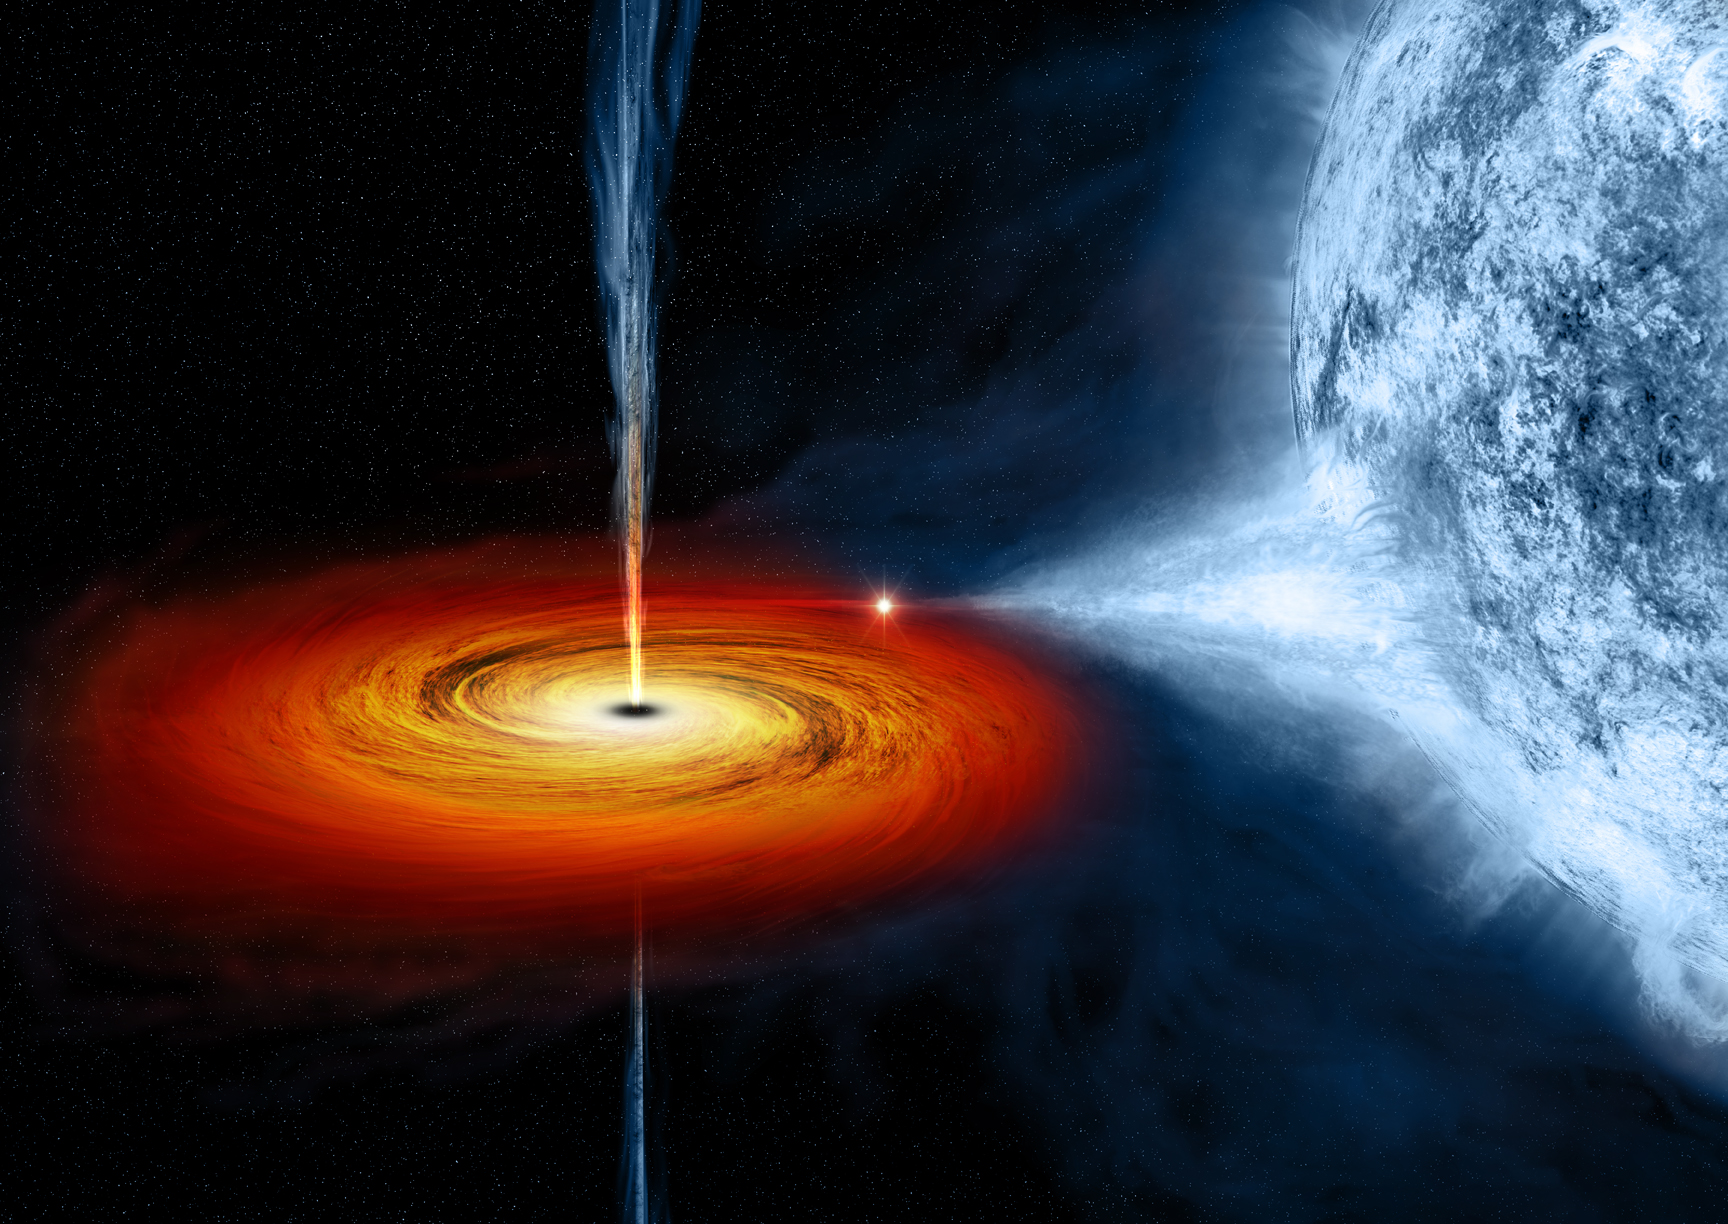
\includegraphics[width=\linewidth,trim={0 1cm 0cm 9cm},clip]{cygnus}};
%    \framenode[5pt]{image} %
%\end{tikzpicture}
%\caption[Artist's impression of a \acs{LMXB}]{An artist's impression of a \ac{LMXB}, showing on a right a companion star from which matter is streaming via Roche-Lobe overflow onto an accretion disk on the left. The inner regions of the disc show jet formation, spewing energy into the surrounding environment. Adapted from \citet{cygnusx1}.}\label{fig:lmxb}
%\end{figure}
%
%
%\subsection{Black Holes \& Neutron Stars}
%\label{sec:intro_bh_ns}
%With accretion onto white dwarfs beyond the scope of this project, the focus turns to black holes and neutron stars. The former were predicted as far back as  \citeyear{schwarzschild1916gravitationsfeld}, and in contrast to neutron stars show no surface, but instead an event horizon -- the innermost boundary beyond which particles can not escape the gravitational pull of the black hole \citep{schwarzschild1916gravitationsfeld}. Compact objects are thought to be formed during the collapse of star in a supernova, although some theories predict accretion onto white dwarfs as a possible channel for neutron star creation. Neutron stars are prevented from further gravitational collapse by neutron degeneracy pressure, provided the mass remains under the Tolman–Oppenheimer–Volkoff limit of approximately $3M_\odot$ \citep{oppenheimer1939massive, rhoades1974maximum}. With strong magnetic fields, such objects can accelerate particles to near-relativistic speeds. Should the magnetic axis be misaligned with respect to the rotation axis of a neutron star, then this can lead to pulsars, objects showing pulsed emission due to the rapid rotation of highly luminous beams.\\
%
%The surface of neutron stars causes some distinct changes in observed emission features. Typically the energy spectrum of such systems will show an extra soft component resulting from surface emission, taking the shape of a comptonised blackbody \citep{done2007modelling}. The extra soft seed photons also affect the higher energies in the resulting spectrum due to their contribution to the illumination of the hot inner flow. Next to the additional component in the energy spectra, neutron star surfaces can lead to additional effects not seen in black holes. Occasionally X-ray bursts in which the observed flux rapidly increases are seen originating from these objects, lasting from seconds to minutes. Bursters can show two types of bursts, type~I bursts resulting from thermonuclear fusion on the surface of neutron stars, and type~II bursts resulting from accretion instabilities. Occasionally  type~I bursts will show burst oscillations, presumed to originate from the rotational modulation of a hot spot on the surface of a neutron star \citep{watts2012thermonuclear}. These burst oscillations provide a means to determine the spin frequency of the central compact object (pulsar periods being another) \citep{chakrabarty2003nuclear}.
%
%\subsection{Accretion}
%There are a number of specific radii which are important to the accretion process. Starting from the centre of a compact object, these radii are often expressed in terms of the  gravitational radius $r_g=GM/c^2$, with $M$ the mass of the central object. For black hole \acp{LMXB} the most important limit is the event horizon. For non-rotating black holes, this is known as the Schwarzschild radius, located at $2r_g$ \citep{schwarzschild1916gravitationsfeld}. White dwarfs and neutron stars however have surfaces rather than event horizons, affecting the emission from these inner regions. The rotation of a neutron star creates a boundary layer at which the angular velocity of accretion disk must decrease to match that of the neutron star, and is the point at which most kinetic energy is released \citep{frank2002accretion, done2007modelling}. This difference between black holes and the other compact objects is thought to play an essential role in the observed emission of such systems \citep[e.g.][]{ghosh1978disk,shakura1988theory,popham2001accretion}. Further out, the strong gravitational fields of compact objects affect the stability of the inner orbits, resulting in the \ac{ISCO} \citep{misner1973gravitation}. Located at $6r_g$ for non-rotating objects, this boundary presents the innermost limit at which an accretion disk can truncate. White dwarfs and neutron stars can truncate a disk further away depending on the strength of their magnetic field. Within the so-called Alfv\'en radius, matter is expected to flow along magnetic field lines towards the central object \citep{lamb1973model}. Finally, there is the truncation radius of the accretion disk, which varies over time depending on the state of an object. To understand the background behind the various states, a brief overview of common analysis techniques is needed.\\
%
%\section{Common Techniques}
%\label{sec:commontechniques}
%
%\subsection{Energy Spectra}
%Since the discovery of the first extra-terrestrial X-ray source Sco X-1 \citep{giacconi1962evidence} methods have been developed to study these sources. Perhaps the most obvious technique is the energy spectrum, providing information on the relative contributions of various components. Fig.~\ref{fig:bh_sp} shows an illustration of a simple black hole energy spectrum including various components, with Fig.~\ref{fig:ns_sp} showing the same for a neutron star. Denoted within the graphs are $BB$ the multicolour disk blackbody, $PL$ the power law emitted by the corona, $FL$ the fluorescent iron line produced by hard coronal photons reflecting off the disk, and for the neutron stars $BLBB$, the boundary layer blackbody. While extremely simplified versions of energy spectra, especially the reflected component, they show the general shapes of the main components. While energy spectra provide a great deal of information on various components, the rapid change in relative strength of these components is difficult to parametrise. As such, the schematic representation of an black hole energy spectrum as given in Fig.~\ref{fig:bh_sp} represents a just a single spectral state of the system, in this case a \ac{SS}. Also, while modelling spectra can be done to some accuracy for single and even multiple observations of the same object, it remains difficult to model an entire population of \acp{LMXB}.\\
%
%\subsection{\NoCaseChange{\acl{HI}} Diagrams}
%In order to be able to compare \acp{LMXB} with each other and study spectral evolution throughout an outburst, \ac{HI}~diagrams were developed, showing the total intensity of an observation against the hardness of an energy spectrum. This latter term refers to the ratio of fluxes measured in two energy bands, with higher over lower energies, similar to how colours work in optical astronomy using Johnson photometry. Parametrising changes in the energy spectrum with hardness provides an model-independent parametrization of the spectral shape, allowing the spectral evolution to be traced. Fig.~\ref{fig:bh_hi} shows an schematic diagram of a \ac{HI}~diagram for a black hole, with abbreviations denoting the canonical black hole states. Starting on the right side of the diagram is the \acf{HS}, transitioning in the top into the \acf{HIMS}, the \acf{SIMS}, and then on the left the \acf{SS}, before transitioning back through the \ac{SIMS} and \ac{HIMS}. The energy spectral evolution through these states is linked to geometric changes over long time scales. While in the hard state, the disk is thought to be truncated far from the compact object, moving inwards while transitioning into the soft state. The changes in geometry strongly affect the energy spectrum. Where in the hard state the disk blackbody is weak in comparison to the hard powerlaw, in the soft state the disk blackbody dominates with the powerlaw reducing in strength and getting softer. This can be understood in terms of the available soft seed photons from the disk. In the soft state a large fraction of disk blackbody photons are upscattered to higher energies due to their close proximity to the corona, but in the hard state this fraction decreases.\\
%
%\subsection{\NoCaseChange{\acl{ECC}} Diagrams}
%Although \ac{HI}~diagrams proved useful in describing the evolution of black holes, the evolution of neutron stars is best traced in a colour-colour diagram. To prevent confusion in successive terminology, this will be referred to as a \ac{ECC}~diagram. By analogy with the hardness parameter defined earlier, a softness parameter is defined, probing lower energies. This allows for a classification scheme based on a wider range in spectral shapes. Fig.~\ref{fig:ns_atoll} and \ref{fig:ns_z} display such diagrams, showing \ac{ECC}~diagrams for two types of typical neutron star \acp{LMXB}, respectively classified as an atoll and a Z~source \marginpar{The tropical names -- atolls, banana etc.~-- originate from the shape of their \ac{ECC}~tracks. Unfortunately this exotic theme was \\ not extended to Z~sources\ldots}. The clear distinction in \ac{ECC}~shapes and rapid variability properties, not to mention the high luminosity of Z sources, initially resulted in this division, but later research showed both types of objects could show similar tracks in the \ac{ECC}~diagram \citep{muno2002z,gierlinski2002comment}. With atolls showing a broad range of luminosities, they remain significantly lower than the luminosities of Z sources, radiating at near Eddington luminosity. The atoll \ac{ECC}~diagram is used to classify the spectral evolution of neutron stars by dividing the track into components, as denoted in Fig.~\ref{fig:ns_atoll}. Starting at the bottom are the banana states, from right to left, the \acf{UB}, the \acf{LB} and the \acf{LLB}. Increasing in hardness is then the \acf{IS} and finally the \acf{EIS}. The luminosity generally increases in the direction the track takes from from the \ac{EIS} to the \ac{LLB}. Transitions between these states can take days to weeks, in contrast to Z~sources where transitions can be in the order of a few days \citep{lin2009spectral}. \\
%
%Switching to the Z~source given in Fig.~\ref{fig:ns_z} reveals several branches distinct from atoll sources, notably the \acf{HB}, \acf{NB} and the \acf{FB} \citep{hasinger1989two}. While the \ac{NB} and \ac{HB} show a smooth evolution in timing properties, the \ac{FB} shows a strong discontinuity in timing features. \citet{kuulkers1994spectral} later subdivided Z~sources into two classes, Cyg-like and Sco-like sources. The \ac{ECC}~diagram given in Fig.~\ref{fig:ns_z} is an example of a typical Cyg-like track, however for Sco-like sources the track is more similar to the shape of a $\nu$. In case of a Cyg-like source the \ac{HB} shrinks and tilts towards the \ac{NB} while the \ac{FB} expands up to the top right. This change in tracks has been to be linked to difference in magnetic fields \citep{psaltis1995x}.\\
%
%%\enlargethispage{2\baselineskip}
%\subsection{Power Spectra}
%In order to capture the timing properties of sources, power spectra can be used. Obtained from Fourier transforms, power spectra vary significantly between spectral states -- whether for black holes or neutron stars. Black hole power spectra typically show a number of features, as displayed in Fig.~\ref{fig:bh_ps}. Denoted with \acs{BBN} is the broad band noise, forming a roughly triangular shape. Additionally there is a \acf{QPO} alongside its harmonic. The study of \acp{QPO} is a field in itself \citep[see][for an overview]{van2006rapid}, although two broad categories exist to explain the origin of these features -- geometric and intrinsic models \citep{van2016probing}. While standing shocks in the accretion flow or changes in mass accretion rate were invoked as possible models in past years \citep[e.g.][]{chakrabarti1993smoothed,tagger1999accretion}, current studies strongly suggest an geometric origin \citep[see][van den Eijnden, 2016, in prep]{heil2015inclination,motta2015geometrical}.\\
%
%Neutron star power spectra show similarities to black hole power spectra, however the presence of a boundary layer and surface make neutron star power spectra more complex \citep{kleinwolt}. Fig.~\ref{fig:ns_ps} gives an schematic example of a neutron star power spectrum, comprising of various components commonly fitted with Lorentzians denoted here with $L$'s. Evolution though spectral states, whether in banana states, or the branches in Z~sources, is tied strongly to changes in the power spectrum -- with components rising and falling in strength but also shifting in frequency. Previous studies comparing neutron star with black hole power spectra provide a way to describe various components \citep[e.g.][]{van1994similarities,wijnands1999broadband,sunyaev2000fourier}, yet a method by which to describe the spectral evolution of \acp{LMXB} in a model-independent fashion remains elusive.\\
%
%\subsection{\NoCaseChange{\acl{PCC}} Diagrams}
%The difficulties in tracking the timing evolution of \acp{LMXB} led \citet{heil2015power} to develop \acf{PCC} diagrams. Inspired by \ac{ECC}~diagrams, \ac{PCC}~diagrams plot ratios of integrated power, or variance, of various frequency bands. Fig.~\ref{fig:bh_pc} shows a schematic example of a \ac{PCC}~diagram, with $PC1$ showing the ratio of the variance in frequency band $C$ over $A$ on the horizontal axis, and $PC2$ showing the ratio of the variance in $B$ over $D$. In this case, the frequency bands $A-D$ refer to consecutive frequency bands in the power spectra, from low to high frequencies. It was discovered that black holes track a near-elliptical path in the \ac{PCC}~diagram, providing a unique manner in which the spectral evolution of black hole systems can be tracked. Denoted in Fig.~\ref{fig:bh_pc} are the approximate positions of the \ac{HS}, \ac{HIMS}, \ac{SIMS} and \ac{SS}, showing a continuous path in evolutionary states. Preliminary research into the \ac{PCC}~track of a neutron star suggested parts of the \ac{PCC}~track differed from black holes power colours. Power colours might well help in establishing a single method by which the spectral evolution of both neutron stars and black holes could be described, providing a strong incentive for further study. \\

\enlargethispage{2\baselineskip}
\section{Motivation}
%Compact objects provide insight into the final stage of stellar evolution, and are key to studying the effect of extreme gravitational fields on matter. Timing analysis allows these innermost regions to be observed at a far larger resolution than photometric analysis can achieve. Combining timing information with spectral information gives a trove of information from which a unique level of detailed insight can be gathered, from accretion theory to the properties of compact objects. A number of studies have been conducted into the timing properties of black holes and neutron stars, but require models to determine the evolution over time. With an entire achieve of \ac{RXTE}~data available, it is now possible to conduct a systematic, model-independent research into the variability of black holes and neutron stars, while testing the applicability of the newly-developed power colour technique.\\

\newpage
\section{Outline}
%While this thesis is intended to be read in full, the possibility arises that earlier sections went unnoticed. As such, this thesis is prefaced by a foreword and several introductory texts. A scientific abstract is available for those working in the field of astronomy, and a popular summary for the general public. With this chapter having presented a brief background to this project, the following chapter describes the methods utilised as part of this thesis. In order to fully understand the intricacies of the data analysis, chapter \ref{sec:methods} also gives information on the \ac{RXTE} spacecraft and the data extraction routines specific to it. Information on the observed population of compact objects can also be found in this section. Chapter \ref{ch:results} then gives a purely phenomenological overview of the results, with interpretations and further discussion provided in chapter \ref{ch:discussion}. The research conducted as part of this thesis is subsequently concluded in chapter \ref{ch:conclusion}. Supplementary information is provided thereafter, in part \ref{part:appendix}. Part \ref{part:appendix} forms the final part of this thesis, in which software details, nomenclature information and graphs pertaining to individual sources are given when inclusion in the main body of text would have prevented a clear flow of information.

%\begin{landscape}
\begin{figure}[H]
%\vspace*{-2cm}
%\hspace*{0.5cm}
\vspace*{-5cm}
\hspace*{0.5cm}
\captionsetup[subfloat]{justification=centering}
\subfloat{%
\begin{minipage}{162pt}
	\begin{tikzpicture}[xscale=2.5,yscale=1.25]
		\coordinate (zero) at (-2,-2);
		\coordinate[right=2 of zero] (a1);
		\draw[very thick,->] (zero) ++ (-0.15,0) -- (2,-2) node[below left] {log E};
		\draw[very thick,->] (zero) ++ (0,-0.15) -- (-2,2) node[above left,rotate=90] {log E$\cdot$F};
		\node[draw,thick,circle,fill=white] at (-2,-2) {A};
		\clip (-2,-2) rectangle (2,2);
		\begin{scope}[shift={(0,0.3)},yscale=1.2]
		%\draw[step=0.1cm,gray,very thin] (-2,-2) grid (2,2);
		%\draw[step=0.5cm,black,thin] (-2,-2) grid (2,2);
		\draw[scale=0.5,domain=-2:3,smooth,variable=\x,thick,dashed] plot ({\x*0.8-3.5},{-\x*\x+1});
		\node[] at (-0.3,-1.5) {\footnotesize FL};
		\draw[scale=0.5,domain=-2.5:2.5,smooth,variable=\x,thick,dashdotted] plot ({\x*0.05-1},{-\x*\x-1});
		\node[] at (-1.6,0.2) {\footnotesize BB};
		%\draw[scale=0.5,domain=-10:10,smooth,variable=\x,thick,solid] plot ({\x},{-0.5*\x-2.5});
		\node[] at (-1.65,-1.5) {\footnotesize PL};	
		\end{scope}
		\draw  plot[thick,smooth, tension=.7] coordinates {(-1.8,-2) (-1.4,-0.4) (0.6,-1.4) (1,-2)};
		\draw[thick]  plot[smooth, tension=.7] coordinates {(-2,0.7) (-1.7,1.8)  (-1.2,0.3) (-0.9,-0.4)(-0.6,-0.6) (-0.5,-0.2) (-0.3,-0.7) (0.6,-1.4) (0.9,-1.7) (1,-2)};
	\end{tikzpicture}
	\label{fig:bh_sp}
\end{minipage}}
\hspace{6cm} % induce horizontal separation
\subfloat{%
\begin{minipage}[c]{162pt}
	\begin{tikzpicture}[xscale=2.5,yscale=1.25]
		\coordinate (zero) at (-2,-2);
		\coordinate[right=2 of zero] (a1);
		\begin{scope}[shift={(0,-0.25)}]
		
		\end{scope}
		\draw[very thick,->] (zero) ++ (-0.15,0) -- (2,-2) node[below left] {Hardness};
		\draw[very thick,->] (zero) ++ (0,-0.15) -- (-2,2) node[above left,rotate=90] {Intensity};
		\node[draw,thick,circle,fill=white] at (-2,-2) {B};
		\draw[thick]  plot[smooth, tension=.7] coordinates {(1.25,-1.75) (0.8,1.2) (-1,1.25) (-1,-0.75) (0.6,-0.6) (1,-1.75)};
		\node at (1.4,0) {\footnotesize HS};
		\node at (0.6,1.8) {\footnotesize HIMS};
		\node at (-0.6,1.8) {\footnotesize SIMS};
		\node at (-1.4,0.2) {\footnotesize SS};
		\node at (-0.6,-1.2) {\footnotesize SIMS};
		\node at (0.55,-1) {\footnotesize HIMS};
	\end{tikzpicture}
\label{fig:bh_hi}
\end{minipage}}

\hspace*{0.5cm}
\subfloat{%
  \begin{minipage}{162pt}  
	\begin{tikzpicture}[xscale=2.5,yscale=1.25]
		\coordinate (zero) at (-2,-2);
		\coordinate[right=2 of zero] (a1);
		\draw[very thick,->] (zero) ++ (-0.15,0) -- (2,-2) node[below left] {log $\nu$};
		\draw[very thick,->] (zero) ++ (0,-0.15) -- (-2,2) node[above left,rotate=90] {log $\nu\cdot$P};
		\node[draw,thick,circle,fill=white] at (-2,-2) {C};
		\draw[thick,dashed] (-2,-0.8) node (v1) {} -- (-0.1,0.4) -- (1.4,-0.7) node (v2) {};
		\clip (zero) rectangle (2,2);
		\draw[thick,dotted]  plot[smooth, tension=.7] coordinates {(-0.8,-2) (-0.5,-1.6) (-0.3,0.9) (-0.1,-1.6) (0.3,-2)};
		\node at (-0.7,-1.2) {\footnotesize QPO};
		\draw[thick,dotted]  plot[smooth, tension=.7] coordinates {(-0.2,-2) (0.1,-1.6) (0.2,-0.3) (0.3,-1.6) (0.6,-2)};
		\node[right] at (0.3,-1.2) {\footnotesize Harmonic};
		\node at (-1.7,-0.9) {\footnotesize BBN};
		\draw[thick]  plot[smooth, tension=.7] coordinates {(v1) (-0.6,0.3) (-0.3,1.8) (-0.1,0.6) (0.1,0.4) (0.2,0.6) (0.4,0.1)  (v2)};
\end{tikzpicture}
\label{fig:bh_ps}
\end{minipage}}
\hspace{6cm} % induce horizontal separation
\subfloat{%
  \begin{minipage}[c]{162pt}
	\begin{tikzpicture}[xscale=2.5,yscale=1.25]
		\tikzset{lor/.style={thick, smooth, dotted, /pgf/fpu,/pgf/fpu/output format=fixed}}
		\coordinate (zero) at (-2,-2);
		\coordinate[right=2 of zero] (a1);
		\draw[very thick,->] (zero) ++ (-0.15,0) -- (2,-2) node[below left] {$PC1$};
		\draw[very thick,->] (zero) ++ (0,-0.15) -- (-2,2) node[above left,rotate=90] {$PC2$};
		\node[draw,thick,circle,fill=white] at (-2,-2) {D};
		\clip (-2,-2) rectangle (2,2);
		\begin{scope}[xscale=1,yscale=0.8]
		%\draw[step=0.1cm,gray,very thin] (-2,-2) grid (2,2);
		%\draw[step=0.5cm,black,thin] (-2,-2) grid (2,2);
		\fill[top color=black, bottom color=black!20,shading=axis,shading angle=45,rotate around={-45:(0,0)}] (0,0) ellipse (2cm and 1cm);
		\fill[white,rotate around={-45:(0,0)}] (0,0) ellipse (1.5cm and 0.5cm);

		\node[] at (0.6,1.1) {\footnotesize HS};
		\node[] at (1.6,-1.5) {\footnotesize HI};
		\node[] at (-0.3,-1.3) {\footnotesize SI};
		\node[] at (-1.65,0.5) {\footnotesize SS};

		\coordinate (c) at (0,0);

		\begin{scope}
		\clip[rotate around={-45:(0,0)}] (0,0) ellipse (2.25cm and 1.25cm);
		\draw[very thick,black!70,dashed] (c) -- +(-6:5);
		\draw[very thick,black!70,dashed] (c) -- +(114:5);
		\draw[very thick,black!70,dashed] (c) -- +(138:5);
		\draw[very thick,black!70,dashed] (c) -- +(-168:5);
		\draw[very thick,black!70,dashed] (c) -- +(-66:5);
		\end{scope}
		\end{scope}
	\end{tikzpicture}
  \label{fig:bh_pc}
  \end{minipage}}
\caption[Common diagrams for black holes]{%
\emph{Common diagrams for black holes} \spacedlowsmallcaps{upper left (A)} A schematic representation of possible energy spectral components, plotted in terms of energy times flux. The disk blackbody $BB$ is denoted by the dashed line, the powerlaw $PL$ by the lower solid line, the fluorescent iron line $FL$ by the dashdotted line, and the total in the upper solid line. With the energy spectra varying over time, these components can pivot and change significantly in intensity \citep[for a full review see][]{gilfanov2014observational}. 
\spacedlowsmallcaps{upper right (B)} A sketch of a \ac{HI}~diagram, showing the general path along which black holes transition. The regions corresponding to canonical spectral states are given in the diagram, with the \acf{HS}, the \acf{HIMS}, the \acf{SIMS} and the \acf{SS} \citep{altamirano}. While in this diagram the transition through the soft states is represented by a smooth line, it commonly is more jagged.
\spacedlowsmallcaps{lower left (C)} A representative power spectrum showing common components, with the broad band noise ($BBN$), a \acf{QPO} and its associated harmonic. Based on \citet{pahari2013comparison}.
\spacedlowsmallcaps{lower right (D)} A schematic \ac{PCC}~diagram, showing the general trend of black hole power colour values. Sources transition along the oval shape, through the various spectral states delineated by the dotted lines. Abbreviations correspond to those adopted in the \ac{HI}~diagram in the upper right plot. The area with no labeling is an overlap of hard and soft states, in which observations can be distinguished with hardness or \acf{RMS} values. Based on \citet{heil2015power}.
}\label{fig:bh_graphs}
\end{figure}
\end{landscape}
%\begin{landscape}
\begin{figure}[H]
\vspace*{-5cm}
\hspace*{0.5cm}
\captionsetup[subfloat]{justification=centering}
\subfloat{%
  \begin{minipage}{0.48\textwidth}
	\begin{tikzpicture}[xscale=2.5,yscale=1.25]

		\coordinate (zero) at (-2,-2);
		\coordinate[right=2 of zero] (a1);
		\draw[very thick,->] (zero) ++ (-0.15,0) -- (2,-2) node[below left] {log E};
		\draw[very thick,->] (zero) ++ (0,-0.15) -- (-2,2) node[above left,rotate=90] {log E$\cdot$F};
		\node[draw,thick,circle,fill=white] at (-2,-2) {A};
		\clip (-2,-2) rectangle (2,2);
		\begin{scope}[shift={(0,0.3)},yscale=1.2]
		%\draw[step=1cm,gray,very thin] (-2,-2) grid (2,2);
		\draw[scale=0.5,domain=-2:3,smooth,variable=\x,thick,dashed] plot ({\x*0.8-3.5},{-\x*\x+0.5});
		\node[] at (-1.55,-0.2) {\footnotesize BB};
		\draw[scale=0.5,domain=-2.5:2.5,smooth,variable=\x,thick,dashdotted] plot ({\x*0.05-1},{-\x*\x-2});
		\node[] at (-0.35,-1.7) {\footnotesize FL};
		\draw[scale=0.5,domain=-2.5:3,smooth,variable=\x,thick,dotted] plot ({\x*1.5-1.75},{-\x*\x-1});
		\node[] at (-0.5,-0.4) {\footnotesize BLBB};
		%\draw[scale=0.5,domain=-10:10,smooth,variable=\x,thick,solid] plot ({\x},{-0.5*\x-2.5});
		\draw  plot[thick,smooth, tension=.7] coordinates {(-1.8,-2.5) (-1.4,-0.9) (0.6,-1.9) (1,-2.5)};
		\node[] at (-1.6,-1.6) {\footnotesize PL};
		\end{scope}
	\draw[thick]  plot[smooth, tension=.7] coordinates {(-2,1.4) (-1.7,1.7) (-1.2,0.9) (-0.6,0.6) (-0.5,0.8) (-0.4,0.4)  (0.3,-0.5) (0.8,-2)};

		\node[draw,thick,circle,fill=white] at (-2,-2) {A};
\end{tikzpicture}
\label{fig:ns_sp}
  \end{minipage}}
\hspace{6cm} % induce horizontal separation
\subfloat{%
  \begin{minipage}[c]{0.48\textwidth}
	\begin{tikzpicture}[xscale=2.5,yscale=1.25]
		\coordinate (zero) at (-2,-2);
		\coordinate[right=2 of zero] (a1);
		\begin{scope}[shift={(0,-0.25)}]
		\draw[thick] (0,1.75) ellipse (1.5 and 0.45); %EIS
		\node[] at (0,1.75) {\footnotesize EIS};
		\draw[thick,xshift=-1.5cm,yshift=-1cm] plot [smooth cycle, tension=0.5] coordinates {(0,0.5) (0,2) (1.5,2)}; %IS
		\node[] at (-1,0.5) {\footnotesize IS};
		\draw[thick,rotate=-30,xshift=0.5cm,yshift=-.4cm] (-1,-1) ellipse (0.5 and 0.28);
		\node[] at (-1.125,-0.95) {\footnotesize LLB};
		\draw[thick] (0,-1.25) ellipse (0.6 and 0.25);
		\node[] at (0,-1.25) {\footnotesize LB};
		\draw[thick,rotate around={30:(1.2,-1)}] (1.2,-1) ellipse (0.5 and 0.25);
		\node[] at (1.2,-1) {\footnotesize UB};
		\end{scope}
		\draw[very thick,->] (zero) ++ (-0.15,0) -- (2,-2) node[below left] {Softness};
		\draw[very thick,->] (zero) ++ (0,-0.15) -- (-2,2) node[above left,rotate=90] {Hardness};
		\node[draw,thick,circle,fill=white] at (-2,-2) {B};
	\end{tikzpicture}
\label{fig:ns_atoll}
  \end{minipage}}

\hspace*{0.5cm}
\subfloat{%
  \begin{minipage}{0.48\textwidth}  
	\begin{tikzpicture}[xscale=2.5,yscale=1.25]
		\coordinate (zero) at (-2,-2);
		\coordinate[right=2 of zero] (a1);
		\begin{scope}[shift={(-0.5,-0.25)},yscale=1.8]
		\draw[thick,rotate around={-50:(-0.7,0.7)}] (-0.7,0.7) ellipse (0.45 and 0.15);
		\node[] at (-0.2,0.8) {\footnotesize HB};
		\draw[thick,rotate around={60:(-0.65,-0.2)}] (-0.65,-0.2) ellipse (0.55 and 0.15);
		\node[] at (-1.1,-0.1) {\footnotesize NB};
		\draw[thick,rotate around={30:(0.75,0.15)}] (0.75,0.15) ellipse (1.75 and 0.15);
		\node[] at (1.25,0) {\footnotesize FB};
		\end{scope}
		\draw[very thick,->] (zero) ++ (-0.15,0) -- (2,-2) node[below left] {Softness};
		\draw[very thick,->] (zero) ++ (0,-0.15) -- (-2,2) node[above left,rotate=90] {Hardness};
		\node[draw,thick,circle,fill=white] at (-2,-2) {C};
	\end{tikzpicture}
\label{fig:ns_z}
  \end{minipage}}
\hspace{6cm} % induce horizontal separation
\subfloat{%
  \begin{minipage}[c]{0.48\textwidth}
	\begin{tikzpicture}[xscale=2.5,yscale=1.25]
		\tikzset{lor/.style={thick, smooth, dotted, /pgf/fpu,/pgf/fpu/output format=fixed}}
		\coordinate (zero) at (-2,-2);
		\coordinate[right=2 of zero] (a1);
		\draw[very thick,->] (zero) ++ (-0.15,0) -- (2,-2) node[below left] {log $\nu$};
		\draw[very thick,->] (zero) ++ (0,-0.15) -- (-2,2) node[above left,rotate=90] {log $\nu \cdot$P};
		\node[draw,thick,circle,fill=white] at (-2,-2) {D};
		\draw[thick]  plot[smooth, tension=.7] coordinates {(-1.6,-2) (-1.3,0.0) (-1.1,0.2) (-0.9,0.4) (-0.65,0.1) (-0.5,0.1) (-0.1,-0.2) (0.35,0.35) (0.72,-1)(1.15,-2)};
		\clip (-2,-2) rectangle (2,2);
		\begin{scope}[shift={(-0.5,-0.25)}]
		%\draw[step=0.1cm,gray,very thin] (-2,-2) grid (2,2);
		%\draw[step=0.5cm,black,thin] (-2,-2) grid (2,2);
		\draw[lor] plot (\x-0.75,{1/(3.14*0.1*(1+((1000*\x)/0.1)^2))-2});
		\draw[lor] plot (\x,{3/(3.14*0.1*(1+((\x + 0.25 )/0.1)^2))-2});
		\draw[lor] plot (\x,{1/(3.14*0.1*(1+((\x)/0.1)^2))-3});
		\draw[lor] plot (\x,{1/(3.14*0.1*(1+((0.1*(2*\x-1.5))/0.1)^2))-2.5});
		\node[] at (-0.75,0.7) {\footnotesize $L_b$};
		\node[] at (-0.4,0.85) {\footnotesize $L_h$};
		\node[] at (0.1,0.5) {\footnotesize $L_{low}$};
		\node[] at (0.8,0.8) {\footnotesize $L_u$};
		\end{scope}
	\end{tikzpicture}
\label{fig:ns_ps}
  \end{minipage}}
\caption[Common diagrams for neutron stars]{%
\emph{Common diagrams for neutron stars} \spacedlowsmallcaps{upper left}~\spacedlowsmallcaps{(A)} A schematic representation of an energy spectrum showing the general shape of the main spectral components in terms of energy times flux \citep[see][]{lin2007evaluating}. The abbreviation $BB$ denotes a multicolour disk blackbody, $FL$ a fluorescent iron line, $BLBB$ the boundary layer blackbody and $PL$ a powerlaw, with the total of all components represented by the upper solid line.
\spacedlowsmallcaps{upper right}~\spacedlowsmallcaps{(B)}  A schematic \ac{ECC}~diagram for an atoll source, with various states denoted. Sources transition around the `C' shape, with starting from the lower right the \acf{UB}, \acf{LB}, \acf{LLB}, then the \acf{IS} and \acf{EIS} \citep{kleinwolt}.
\spacedlowsmallcaps{lower left (C)} A schematic Z source \ac{ECC}~diagram, showing the \acf{HB}, the \acf{NB} and the \acf{FB} \citep{kleinwolt}.
\spacedlowsmallcaps{lower right (D)} A simplified power spectrum of an atoll in the \ac{EIS} state showing various commonly fitted Lorentzian components. These components can rapidly change in number, amplitude, and width over time, while shifting in frequency. Sharply peaked components can emerge at the higher frequencies, referred to as kHz \acfp{QPO} \citep[see][]{kleinwolt,marieke}. 
	}\label{fig:ns_graphs}
\end{figure}
\end{landscape}